\documentclass[a4paper,14pt]{article}         % класс документа - статья. Также report, book и др.
\usepackage{geometry}           % пакет для задания полей страницы командой \geometry
\geometry{a4paper, left=3cm,right=1.5cm,top=2cm,bottom=2cm}
%\usepackage[cp1251]{inputenc}   % кодировка текста
%\usepackage{mathtext}           % позволяет использовать русские буквы в формулах
%\usepackage[T2A]{fontenc}       %пакет Т2А необходим для правильного отображения кириллицы и переноса слов
%\inputencoding{cp1251}          % тоже кодировка...
% Для русского
\usepackage[utf8]{inputenc}
\usepackage[T2A]{fontenc}
\usepackage[russian]{babel}
%\usepackage{textcomp}
%\usepackage[unicode]{hyperref}  %создаёт гиперссылки на список литературы в pdf-файле
\usepackage{amstext,amsmath,amssymb}            % пакеты для формул
\usepackage{bm}                 % boldmath - пакет для жирного шрифта
\usepackage[pdftex]{graphicx}   % пакет для включения рисунков в форматах png,pdf,jpg,mps,tif
                                % надо компилировать сразу в pdf
\usepackage{hyperref}			% ссылки
\usepackage{amsfonts}           % греческие символы и, возможно, что-то ещё
\usepackage{indentfirst}        % одинаковый отступ для первого параграфа и всего остального
%\usepackage{cite}               % команда /cite{1,2,7,9} даёт ссылки
\usepackage{multirow}           % пакет для объединения строк в таблице: надо указать число строк и ширину столбца
\usepackage{array}              % нужен для создания таблиц
\linespread{1.3}                % полтора интервала. Если 1.6, то два интервала

% Подписи рисунков
\usepackage[font=Large,labelfont=bf]{caption}
\DeclareCaptionLabelSeparator{defffis}{ --- }
\captionsetup{justification   = raggedright,
			singlelinecheck = false,
			labelsep=defffis,}
\usepackage{subcaption}

% Шрифты секций
\usepackage{sectsty}
\sectionfont{\centering\fontsize{14}{15}\selectfont}
\subsectionfont{\fontsize{14}{15}\selectfont}
\subsubsectionfont{\fontsize{14}{15}\selectfont}

% Внутри секции картинки
\usepackage[section]{placeins}

% рекомендуется при использвоании biblatex
\usepackage{csquotes}
%\bibliographystyle{unsrt}
\bibliographystyle{ugost2008}

\usepackage[%
autolang=other,       
bibencoding=utf8,
sorting=none, % Name,Title,Year или sorting=none.
maxbibnames=4, % Максимальное число авторов в списке литературы.
minbibnames=2, % Число авторов, отображаемое при сокращении.
style=gost-numeric,
backend=biber]{biblatex}
\addbibresource{cite/Literature.bib}

\usepackage{xcolor}
%\titleformat{\section}[block]{\Large\bfseries\filcenter}{}{1em}{}
\pagestyle{plain}               % номерует страницы
\parindent=1.25cm				% правильный размер красных строк
\renewcommand{\theenumii}{\asbuk{enumii}} % списки с русским алфавитом

% Listings
\usepackage{listings}
\usepackage{color}

\definecolor{codegreen}{rgb}{0,0.6,0}
\definecolor{codegray}{rgb}{0.5,0.5,0.5}
\definecolor{codepurple}{rgb}{0.58,0,0.82}
\definecolor{backcolour}{rgb}{0.95,0.95,0.92}

\lstdefinestyle{mystyle}{
	backgroundcolor=\color{backcolour},   
	commentstyle=\color{codegreen},
	keywordstyle=\color{magenta},
	numberstyle=\tiny\color{codegray},
	stringstyle=\color{codepurple},
	basicstyle=\footnotesize\ttfamily,
	breakatwhitespace=false,         
	breaklines=true,
	%postbreak=\mbox{\textcolor{red}{$\hookrightarrow$}\space},                 
	captionpos=b,                    
	keepspaces=true,                 
	numbers=left,                    
	numbersep=5pt,                  
	showspaces=false,                
	showstringspaces=false,
	showtabs=false,                  
	tabsize=2,
}

\lstset{style=mystyle}

\usepackage{icomma} % для отображения запятой как разделителя целой и дробной частей числа

% Рыжие заметки
\newcommand{\sic}[1]{\LARGE\color{orange}{#1}\color{black}\Large}

\begin{document}
\def\figurename{Рисунок}
\section*{Аннотация}

	\Large
Темой данной работы является поиск новых лекарств, возможных побочных эффектов и неспецифичных взаимодействий между биомолекулами. Целью работы являлось построение гибкого программного протокола, способного на основе референсных данных об эффективных и безопасных для человека лекарствах построить поиск наиболее сходного лиганда/мишени/комплекса на основе соответствующих входных данных. В результате такой протокол был создан, проверен и задокументирован. 
\if 0 В него также был внедрен пользовательский интерфейс через запуск в командной строке с нужными ключами. 
\fi
Протокол позволяет осуществлять поиск наиболее близких референсных лигандов по их структуре и SMILES идентификатору с помощью молекулярных отпечатков, поиск наиболее схожих референсных белков по их аминокислотным последовательностям и 3D-структурам, а также поиск наиболее похожих комплексов референсных лигандов по структуре связывающих карманов. В будущем протокол может дополняться другими способами вычисления подобия, а также на его основе может строиться более сложный поиск, например, с помощью методов машинного обучения.

\setcounter{page}{2}            % Нумерация страниц начинается с "2"

\newpage                        % Начинает текст с новой страницы
\tableofcontents                % Автоматическое создание оглавления по названиям разделов, подразделов и т.п.

\newpage
\section*{Определения, обозначения и сокращения}

\textbf{Лиганд}~--- в биологии это химическое соединение, обычно малая молекула, которая образует комплекс с той или иной биомолекулой-мишенью (чаще всего белком) и производит, вследствие такого связывания, те или иные биохимические, физиологические или фармакологические эффекты.

\textbf{Мишень}~--- биомолекула, с которой может связываться молекула-лиганд, производя некоторый биологический эффект в организме.

\textbf{FDA}~--- американское управление по санитарному надзору за качеством пищевых продуктов и медикаментов (англ. Food and Drug \linebreak Administration) ~--- служба, занимающаяся контролем качества лекарственных препаратов, пищевых продуктов и других категорий товаров, а также осуществляющая контроль за соблюдением законодательства и стандартов в этой области. 

\textbf{Метрика подобия или схожести}~-- способ сопоставить всем парам объектов из входных данных одного типа некоторые безразмерные числа, позволяющие судить о схожести этих объектов.

%\textbf{Биологическая молекула (биомолекула)}~--- 
\textbf{а/к}~--- аминокислота.

\textbf{АКП}~--- аминокислотная последовательность.

\textbf{ID}~--- идентификатор.

\textbf{БД}~--- база данных.

\textbf{ПМ}~--- программный модуль.

\textbf{ПП}~--- программный пакет.

\textbf{GPCR} --- рецепторы, сопряженные с G-белком (англ. G-protein-coupled receptors).
\if 0
\color{gray}
\textbf{ТМ} --- трансмембранный участок

\textbf{МГ} --- моделирование по гомологии

\textbf{МД} --- молекулярная динамика
\color{black}
\fi
\newpage
\section{Введение}
Математическое моделирование и вычислительные методы давно стали неотъемлемой частью исследований в биологии и медицине, причем налицо тенденция к росту важности и востребованности таких методов и в фундаментальной науке, и в приложениях. Так, в современной фармакологии высокопроизводительный виртуальный скрининг является важнейшим этапом отсева молекул-кандидатов перед дорогостоящими клиническими испытаниями. Использование компьютерных расчетов позволяет значительно сократить количество затрачиваемых на поиск лекарства времени и ресурсов.

Одним из методов поиска и отсева кандидатов является сравнение с уже известными лекарствами, имеющими положительные и побочные эффекты. Таким способом можно производить поиск как новых мишеней для уже известных лекарств, так и по известным мишеням находить новые лиганды для них. Кроме поиска лекарства, такие исследования могут помочь в нахождении побочных эффектов и ранее неизвестных последствий одновременного использования нескольких препаратов. Однако, насколько нам известно, сейчас не существует публично доступного программного модуля или пакета, позволяющего искать кандидатов в новые лекарственные средства с использованием широкого спектра различных метрик подобия.

\textbf{Целью} данной работы являлось построение такого гибко настраиваемого программного протокола для поиска неспецифичных взаимодействий между лигандами и мишенями. 

Для достижения этой цели были предложены следующие этапы:
\begin{enumerate}
	\item извлечь из доступных баз данных биологических соединений необходимую информацию о подтвержденных FDA лекарствах, соответствующих лигандах и мишенях, и реализовать это в программном коде;
	\item создать функции для конвертации данных одной молекулы в требуемые сторонними программами форматы;
	\item создать функции для сравнения одного элемента входных данных с одной подтвержденной FDA записью;
	\item реализовать поиск по референсным данным наиболее подходящих в терминах различных метрик подобия для лигандов/мишеней/комплексов.
\end{enumerate}

\subsection{Обзор литературы}
\subsubsection{Полифармакология}
При разработке лекарств важно добиться селективности, избавившись от побочных действий. Именно эта парадигма <<одно лекарство~--- одна мишень>>, так называемая таргетированная терапия, до недавнего времени широко использовалась в фармакологии. С другой стороны, в последнее время стала осознаваться важность полифармакологии, которая означает множественное, но специфичное воздействие лекарства на многие мишени, позволяющее добиться синергетического эффекта и более эффективного лечения комплексных заболеваний, таких как рак\cite{Anighoro2014}. 

При этом полифармакология может выгодно отличаться от комбинирования нескольких лекарств, так как:

(а) единственная молекула обычно имеет более предсказуемую и безо\-пасную фармакокинетику; 

(б) часто действующие на несколько мишеней лекарства имеют \linebreak {б\textbf{о}льшую} эффективность на поздних стадиях заболевания; 

(в) не нужно учитывать эффекты перекрестного взаимодействия лекарств, которые, являясь негативными, переносятся хуже в случае комбинационной терапии; 

(г) при прочих равных  вероятность привыкания к единственному лекарству меньше, чем к хотя бы одному из набора лекарств \cite{Anighoro2014}.

Стоит заметить, что каждый белковый домен в среднем содержит 3--5 связывающих карманов достаточного размера для связывания с типичными малыми лигандами\cite{Skolnick2015}. Таким образом, существует возможность выбрать новый карман, отличный от ранее использовавшихся, для разработки лекарства. К тому же, количество видов связывающих карманов со статистически значимыми различиями, по оценке, не превышает 400 \cite{Skolnick2015}, что позволяет считать полифармакологическую картину взаимодействий лиганд-мишень неизбежной, и потому более перспективной, чем таргетированная.

Новая парадигма подчеркивает важность поиска всевозможных пар взаимодействий лиганд-мишень. Такой анализ может аккумулировать результаты уже известных связей, приводя к построению сложных сетей \cite{Anighoro2014}, но важнее уметь предсказывать такие взаимодействия. Так как перебор и оценка силы всех взаимодействий лиганд-мишень \textit{in vivo} и \textit{in vitro} является непрактичной, в этом направлении активно развиваются компьютерные методы \cite{Chaudhari}.

\subsubsection{Неспецифичные взаимодействия и их поиск}
Неспецифичные взаимодействия~--- дополнительные взаимодействия выбранного лиганда/мишени с другими, кроме основных, мишенями/лигандами. Одной из главных проблем в поиске таких взаимодействий исходя из структуры является то, что часто эти связи в большой степени определяются подвижными частями рецептора, которые сложно или невозможно исследовать с достаточной атомарной точностью \cite{Loving}.

Принципиально, структурный поиск субъектов неспецифичного взаимодействия может осуществляться по структуре: (а) мишени; (б) лиганда; (в) связывающего сайта \cite{Rognan2010}.

(а) При поиске возможных лигандов по известной структуре мишени, обычно воспроизводится процесс современного дизайна лекарств, а именно высокопроизводительный скрининг по базе возможных лигандов. Таким образом, в сущности, оценивается, насколько сложно найти лиганд для этой мишени. 

Схожесть мишеней можно оценивать по их АКП (1D\,--\,мера) или по структурным особенностям (3D\,--\,меры). Вычисление 3D\,--\,мер часто бывает ресурсоемким, но этот процесс можно ускорить, используя поиск по так называемым <<горячим точкам>>, то есть набору мест на поверхности мишени, где максимальна энергия связывания с потенциальным лигандом \cite{Hall2015}. Это напоминает концепцию фармакофорного поиска, то есть нахождения определенных пространственных и электронных структур, особенно энергетически выгодных для связывания лиганда.

(б) Поиск по структуре лиганда близок по своей сути к понятию лекарственной репозиции, заключающемуся в поиске новых мишеней и применений для лекарств, которые уже выпущены на рынок. Это позволяет сократить расходы на преклиническую стадию и оптимизацию \cite{Hall2015, March-Vila2017}.

Для нахождения сходства лигандов по их топологической структуре могут использоваться молекулярные отпечатки нескольких типов. Существуют разнообразные принципы построения отпечатков: могут хэшироваться различные топологические пути, могут искаться фармакофоры или определенные подструктуры, существуют и способы с использованием только текста SMILES \cite{Cereto-Massague2015}. В получающихся для двух лигандов битовых строках вычисляется относительное количество общих битов\,--\,свойств, что и приводит к оценке степени подобия структур (см. коэффициент Танимото в разделе \ref{sec:tanim}). 

Преимуществом молекулярных отпечатков является относительная быстрота их построения и возможность предварительного их вычисления для всех элементов референсных данных. После этого для сравнения с новым элементом достаточно лишь раз посчитать отпечаток для него, а также пройти по базе данных (БД) для вычисления коэффициентов Танимото, что принципиально является просто вычислением бинарных <<И>> и <<ИЛИ>> для битовых строк. Однако, для эффективной работы принципа молекулярных отпечатков нужно среди всего их множества выбирать наиболее подходящие к конкретному классу сравниваемых соединений \cite{Cereto-Massague2015}.

(в) Связывающие карманы могут сравниваться по различным характеристикам, таким как геометрические и физико-химические свойства поверхности мишени, профили взаимодействия или структура остова \cite{Ehrt2016}. Соответственно, точность и ресурсоемкость различных методов варьируются в широких диапазонах.

Полости могут описываться разными способами. Например, как трехмерный граф из вершин-атомов, соединенных ребрами-длинами. Или же как облако точек, то есть чисто геометрически. В этих моделях могут выделяться основанные на фармакофорном принципе черты, которые в дальнейшем позволяют значительно ускорить поиск. Один из наиболее затратных в вычислениях, но и чувствительных методов~--- построение карт электронной плотности \cite{Ehrt2016}.

Кроме того, нахождение полостей само по себе сложная задача, к которой существует несколько подходов. Подавляющее большинство способов нахождения полостей подразумевает модель твердых шаров для структуры молекул, что сводит задачу преимущественно в область обработки геометрических данных \cite {Krone2016}, хотя часто используются и вычисления пробных потенциалов с построением соответствующих карт и дальнейшим выделением областей методами вычислительной математики (например, методом Нелдера — Мида).

Существуют методы, основанные на построении сетки, которые благодаря совершенствованию вычислительных возможностей в последнее время стали вновь широко использоваться. Их преимущество в практически неограниченном росте точности при уменьшении размера сетки. Недостаток -- в <<прямоугольности>> и дискретности сетки, которые, впрочем, с помощью различных ухищрений могут сглаживаться.

Другой класс методов основан на диаграммах Вороного и триангуляциях Делоне \cite{Aurenhammer1991}, которые позволяют автоматически избавиться от дискретности и сильной зависимости точности построения от ресурсоемкости, а также более применимы для анализа структур в динамике. Недостаток этого класса состоит в неуниверсальности замены атомов твердыми шарами, а также сложности обработки построенных диаграмм.

Еще один класс методов использует, по сути, множественное <<встраивание>> пробника в структуру. В простейшем случае пробником является сфера, ее радиус может уменьшаться до достижения нужной точности. Преимущество этого класса в возможности автоматически учитывать размер лиганда, задавая размер пробника порядка размера лиганда. Проблема такого рода методов в сильной зависимости от размера молекул и недостаточной точности \cite{Krone2016}.

Комбинация различных методов из вышеперечисленных позволяют использовать их преимущества при уменьшении эффекта недостатков.
%\cite{Cabrera}
%\cite{Brylinski}
%\cite{Govindaraj2018}
\subsubsection{Актуальность}
Большинство существующих работ по поиску неспецифичных взаимодействий для построения соответствующих предсказаний рассматривают преимущественно один метод вычисления подобия \cite{Santos2016, Chartier2017}.
 
Это мотивирует нас на создание протокола, способного использовать несколько различных типов вычисления подобия молекул/комплексов и гибкого к добавлению новых способов.



\newpage
\section{Основное содержание}
\subsection{Общая структура протокола}
Опишем общую структуру протокола (см. рис. \ref{structure}).

Так как для поиска по подобию нужны референсные данные, то необходимо найти их источник. Таким источником могут являться биологические базы данных, содержащие необходимые для оценок сходства входных данных с референсными. Извлекая сведения об подтвержденных FDA лекарствах, можно, используя эту же и другие базы данных биомолекул, получать и сохранять в структурированном виде необходимые для дальнейшего поиска сведения о свойствах референсных лигандов/мишеней и извлекать структурную информацию о них и их комплексах.

После этого с помощью сторонних программных модулей и пакетов для оценки сходства молекул/комплексов и обработки данных, а также собственного модуля достигается цель~--- нахождение списка лигандов/мишеней/комплексов наиболее близких к входным данным.

\begin{figure}[hp]
		\centering{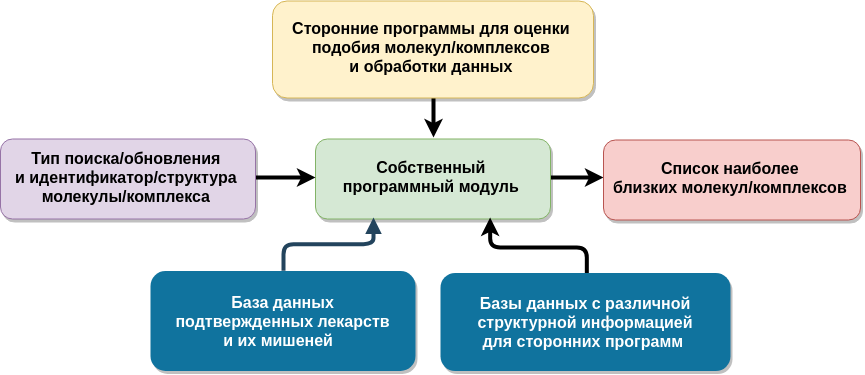
\includegraphics[width=1.0\linewidth]{Drawio/6}} % Вставляем рисунок в полученное "окно" полностью - 100%
		\caption{Общая схема структуры протокола.}
		\label{structure}
\end{figure}

\newpage
\subsection{Материалы и методы исследования}
\subsubsection{Биологические и химические базы данных}
Объем и качество биологических данных растут с каждым годом, что требует эффективных способов их хранения и оперирования ими. С этой целью были созданы, создаются и обновляются биологические базы данных, содержащие самую разнообразную информацию о биологических и биоактивных молекулах, тканях, видах, лекарствах и так далее. Обычно биологические БД имеют свой сайт и реализованный пользовательский интерфейс/API для извлечения информации об отдельных записях и поиску по набору свойств. Записи могут аннотироваться и проверяться автоматически и вручную, от чего часто зависит качество представляемых в биологических БД сведений.

Примерами таких БД являются: 
\begin{itemize}
	\item Drugbank \cite{drugbank}~--- специализируется на подтвержденных FDA и экспериментальных лекарствах; 
	\item Uniprot \cite{uniprot}~--- содержит информацию о белках и протеомах; 
	\item PDB \cite{pdb}~--- состоит из записей о структурной информации биомолекул и комплексов;  
	\item PubChem \cite{pubchem}~--- является более общей химической БД, однако содержит химическую информацию и о биомолекулах, биоактивных веществах. При поиске абсолютно новых лекарств они часто еще не включены в класс биоактивных веществ, так что общие химические БД также используются в биологических исследованиях и приложениях.
\end{itemize}
\subsubsection{Коэффициенты Жаккара и Танимото} \label{sec:tanim}
Для удобства работы с мерами сходства как с числами имеет смысл ввести единообразное для самых разных типов данных определение бинарного коэффициент сходства. Коэффициент Жаккара \cite{Jaccard1901} позволяет для любых двух конечных множеств $A, B$ получить коэффициент подобия $J(A, B)$ по формуле
\begin{equation}
\label{jaccard}
J(A, B) = \frac{|A\cap B|}{|A\cup B|} \in [0, 1].
\end{equation}
Видно, что равенство коэффициента нулю означает полное отсутствие сходства между множествами. Чем больше значение $J(A, B)$, тем выше степень сходства множеств вплоть до полного совпадения при $J(A, B) = 1$.

Частным случаем этого коэффициента является коэффициент Танимото, применяющийся в случае сравнения бинарных множеств $A, B$. Тогда их можно охарактеризовать битовыми векторами $\textbf{a}, \textbf{b}$, и в этом случае \linebreak $T(\textbf{a}, \textbf{b}) \equiv J(A, B) $ из (\ref{jaccard}) можно переписать проще для прямого вычисления:
\begin{equation}
T(\textbf{a}, \textbf{b}) = \frac{\textbf{a}\cdot\textbf{b}}{|\textbf{a}|^2 + |\textbf{b}|^2 - \textbf{a}\cdot\textbf{b}}.
\end{equation}

\subsubsection{Сходство белков по аминокислотной последовательности}
Для вычисления сходства двух АКП обычно используется алгоритм BLAST \cite{ALTSCHUL1990403} или его вариации. Принцип работы алгоритма заключается в поиске выравниваний двух АКП, возможно с пробелами, таким образом, чтобы суммарное сходство $S$, определяемое как сумма весов, взятых из предопределенной матрицы замен (см. рис. \ref{fig:blosum}) для всех выравненных пар а/к и пробелов из двух последовательностей:
	\begin{equation*}
	S = \sum_{i=1}^{L_{align}} M\dot Sub,
	\end{equation*}
	где сумма ведется по всем номерам аминокислот/пробелов в выравнивании, $M$ - матрица замен с учетом замен пробелов/на пробелы, $Sub$ - матрица количеств замен в данном выравнивании каждого типа аминокислот и пробелов на другие аминокислоты/пробелы.
Вначале строятся частичные выравнивания с помощью поиска соответствий в 3 а/к, затем пробуется продлить эти соответствия сначала без пробелов, потом с ними. В итоге, вычисляется коэффициент суммарного сходства и идентичность, определяемая как количество пар одинаковых а/а в выравнивании, а лучшее выравнивание выводится на экран.

Для вычисления сходства белков описанным выше образом по их аминокислотным последовательностям был использован модуль Biopython \cite{biopython}.
\begin{figure}[h] 
	\centering
	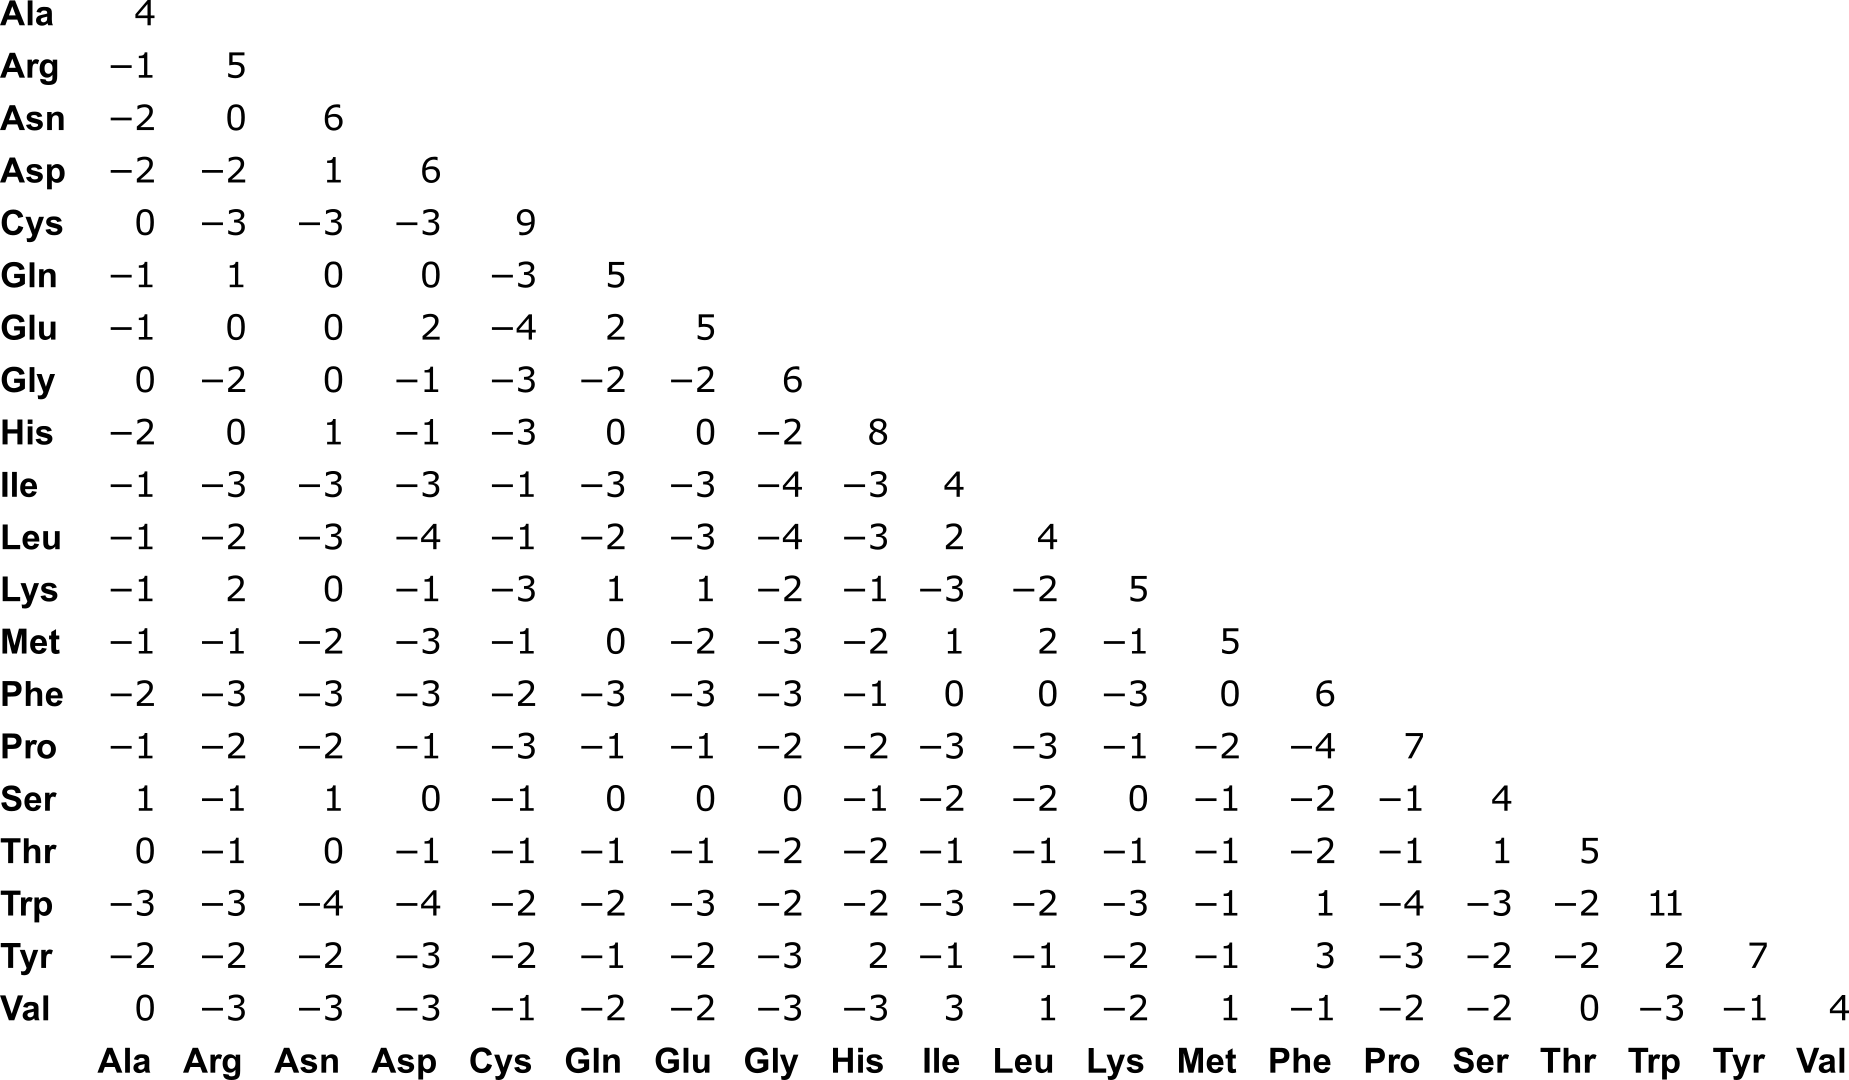
\includegraphics[width=0.8\linewidth]{pictures/BLOSUM62}
	\caption{Наиболее часто используемая в выравниваниях АКП матрица замен BLOSUM62.}
	\label{fig:blosum}
\end{figure}
\subsubsection{Сходство белков по структуре} \label{TM principle}
Чтобы вычислить сходство белков, используя их структуру, использована программа TM-align \cite{TM, TMalign}. Сначала определяется оптимальное наложение двух белков друг на друга, нахождение которого, вообще, является NP-трудной задачей без точного решения \cite{Lathrop1994}, и поэтому обычно требует существенных вычислительных ресурсов. Однако, применяемый в TM-align алгоритм позволяет уменьшить время работы на порядок без потери точности, что и послужило причиной его выбора в качестве основы для этой части протокола.

Для выравнивания структур сначала с помощью динамического программирования определяется выравнивание вторичных структур и строится соответствующая бинарная оценочная матрица. Потом меньший белок <<протягивается>> по большему для беззазорного выравнивания и вычисляется соответствующая оценочная матрица. Матрица для итогового выравнивания берется как средняя первых двух, а выравнивание строится посредством алгоритма динамического программирования. В итоге вычисляется TM-score (англ. Template Modeling score)\cite{Zhang2004, Levitt1998}. 
\begin{equation}
\label{tm-score}
\text{TM-score} = \max\left[\frac{1}{L_{target}}\sum_i^{L_{aligned}}\frac{1}{1+\left(\frac{d_i}{d_0(L_{target})}\right)^2}\right],
\end{equation}
где <<$\max$>> обозначает наилучшее значение после пространственного наложения белков, $L_{target}$~--- количество а/к в целевом белке, сравниваемом с другими; $L_{aligned}$~--- количество а/к в выравненной части двух белков, $d_i$~--- расстояние между $i$-й парой остатков в белках; нормировочный коэффициент $d_0(L_{target}) = 1.24\sqrt[3]{L_{target}-15}-1.8$; сумма производится по парам соответствующих оснований. 

TM-score нормирован таким образом, что его значение не зависит от длин сравниваемых белков. Также из статистических исследований следует, что значение TM-score меньше 0,2 говорит об отсутствии корреляций в структурах, а превышение эмпирической границы в 0,5 означает, что укладки белков практически совпадают \cite{TMalign, Xu2010}. 

Одновременно считается и коэффициент RMSD (англ. Root Mean Square Deviation) %\ref{rmsd}
\begin{equation}
\label{rmsd}
\text{RMSD} = \sqrt{\frac{1}{N}\sum_{i=1}^N \delta_i},
\end{equation}
где $N$~--- количество атомов в первой структуре; $\delta_i$~--- отклонение $i$-го атома от второй структуры.

TM-score считается более подходящим для оценки подобия белков, чем RMSD, так как в отличие от RMSD он не зависит от длин сравниваемых белков (нормируется на полусумму их длин и находится в полуинтервале $(0, 1]$), а также учитывает различные области белков с разными весами, что позволяет получать адекватные результаты для структур с одинаковой глобальной топологией, но небольшими отклонениями по всей длине белка. В случае использования RMSD результат будет подразумевать то, что структуры различны, а TM-score, вероятнее всего, детектирует схожесть \cite{TMalign}.
\subsubsection{Сходство лигандов по структуре}
Мы использовали вычисление молекулярных отпечатков по SMILES (текстовый отпечаток \cite{Weininger1989}) и SDF файлу (топологические пути и поиск подструктур \cite{Cereto-Massague2015}). Нахождение этих отпечатков реализовано с помощью модулей RDkit \cite{rdkit} и Open Babel \cite{openbabel} соответственно. Не представляет сложности при необходимости добавить другие типы и реализации вычисления молекулярных отпечатков, например фармакофорные отпечатки из тех же модулей.

\subsubsection{Сходство сайтов связывания}

Для вычисления подобия сайтов связывания используется программный пакет (ПП) IsoMIF \cite{isomif, Chartier2015}, считающийся одним из лучших для данного вычисления, хотя и вычислительно затратным] \cite{Ehrt2016}.

Суть его работы состоит в нахождении и обработке полостей структуры комплекса лиганд-мишень\cite{Gaudreault2015} Для нахождения пустот используется реализация алгоритма SURFNET \cite{Laskowski1995} (см. рис \ref{fig:cleft}). Этот алгоритм не позволяет выделить именно полости между несколькими молекулами, потому что также помечает внутренние пустоты и углубления в молекулах как полости. При этом поиск производится начиная с наибольших полостей к меньшим, а в большинстве случаев именно наибольшая полость в структуре комплекса и является сайтом связывания с лигандом \cite{Laskowski1995}. 

Принцип нахождения полостей базируется на постепенном вписывании сфер наибольшего радиуса посередине между всеми парами атомов, где каждый из пары берется из отдельной молекулы. Атомы также считаются шарами, с которыми новые сферы не должны пересекаться. Сферы вписываются в структуру до тех пор, пока нельзя будет вписать еще одну минимального заранее заданного радиуса. После этого в центре каждой сферы строится гауссиан, вносящий вклад в общую карту интенсивности, а по суммарной карте интенсивности, из которой по заданному порогу легко выделить поверхность и полости \cite{Laskowski1995}.
\if 0
\begin{figure} 
	\centering
	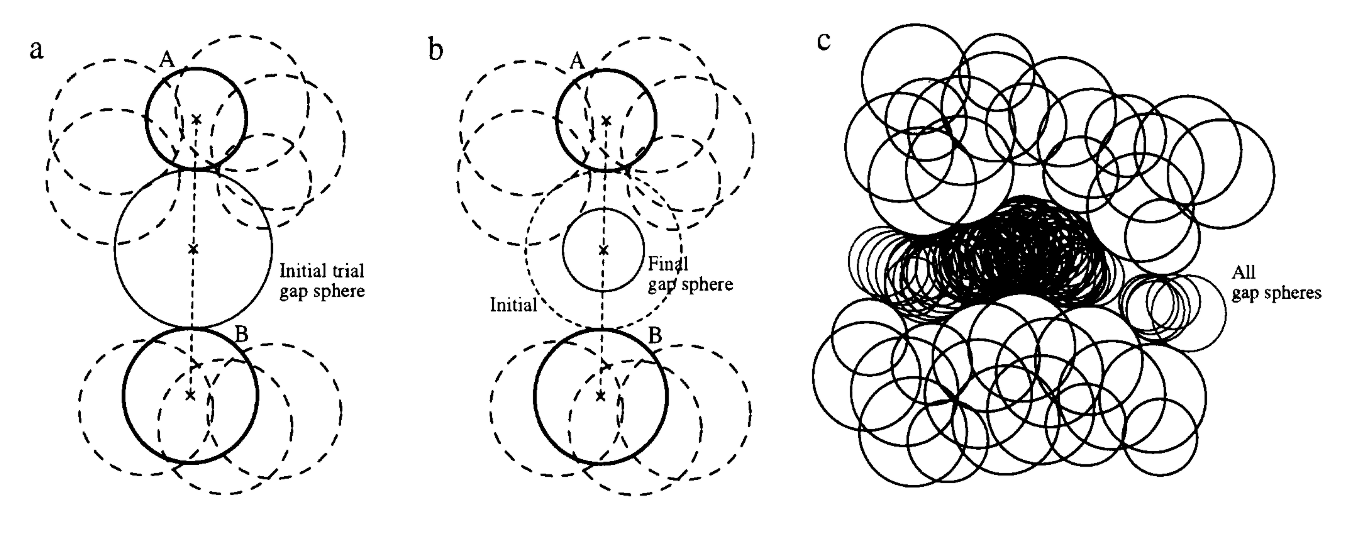
\includegraphics[width=1\linewidth]{pictures/surfnet}
	\caption{Процесс построения сфер алгоритмом SURFNET. (a) ---  \sic{Дописать}}
	\label{fig:surfnet}
\end{figure}
\fi
\begin{figure} 
		\centering
		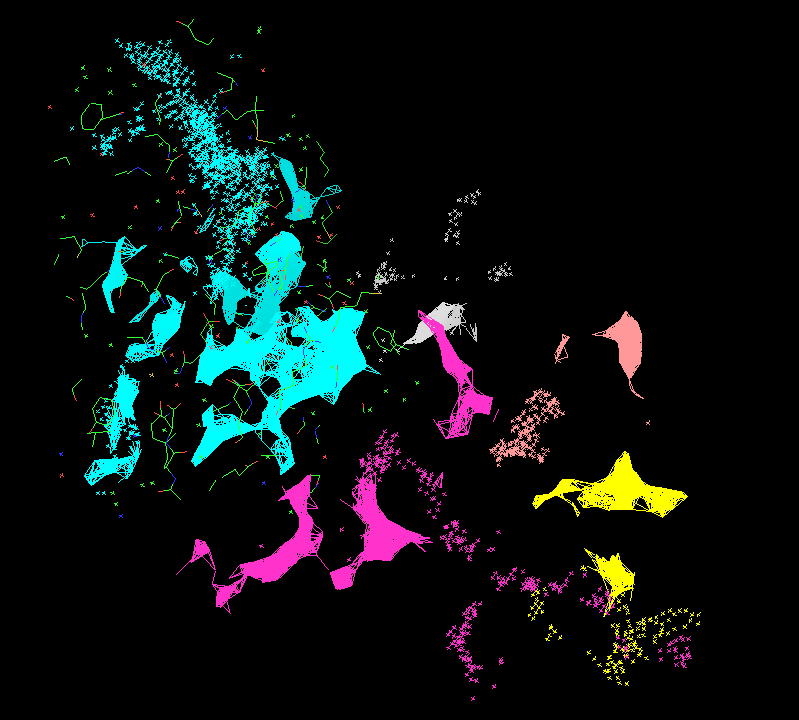
\includegraphics[width=0.6\linewidth]{pictures/clefts}
		\caption{Пять наибольших полостей в структуре 1E8X из БД PDB, найденных с помощью Get Cleft, показаны разными цветами.}
		\label{fig:cleft}
\end{figure}

После этого с помощью встроенной в пакет программы MIF (англ. Molecular Interaction Field) в области сайта связывания строится сетка, в каждом узле которой считаются энергии взаимодействия пробника определенного типа с соседними атомами белка до некоторого радиуса обрезки. Всего используется 6 типов энергий, зависящих от следующих свойств молекулы: гидрофобность, ароматичность, способность быть донором/акцептором водородной связи, положительный/отрицательный электрический заряд. Энергии спадают одинаково и экспоненциально от расстояния, а значения энергий на 1 \AA $\:$ подбираются эмпирически для всевозможных пар из 6 типов энергии и 13 видов атома белка (см. рис. \ref{fig:mif}).

После получения этих сеток для двух сайтов связывания (с 6 значениями энергии в каждом узле) происходит построение графа, у которого вершины обозначают пары узлов сетки, берущихся по одному из сравниваемых структур и имеющих хотя бы один общий из 6 типов энергии больше некоторого порога, то есть является значимым. Ребра в этом графе строятся, если расстояния между соответствующими узлами в двух полостях отличаются менее, чем на 3 \AA. 

Затем в этом графе производится поиск наибольшей клики (полного подграфа) с помощью алгоритма Брона — Кербоша \cite{Bron1973, Tomita2006} и с использованием эвристического наблюдения, что наибольшая клика часто находится одной из первых, так что для значительного уменьшения вычислительной нагрузки проводится только 100 поисков по умолчанию. 

Результат работы алгоритма~--- мера подобия полостей,~--- вычисляется как
\begin{equation}
\text{MSS} = \frac{N_c}{N_a + N_b - N_c},
\end{equation}
где $N_c$~--- количество значимых общих типов взаимодействий у всех вершин в клике, $N_a, N_b$~--- количества значимых типов взаимодействий в узлах сеток для первого и второго белка \cite{Chartier2015}.  

Также в протокол включена возможность использовать TM-score для сравнения структур комплексов. Такая функция в программе TM-align появилась недавно и описание ее работы еще не опубликовано, но, вероятно, она работает по тому же принципу, что и соответствующее сравнение белков (см. раздел \ref{TM principle}).
\begin{figure} 
		\centering
		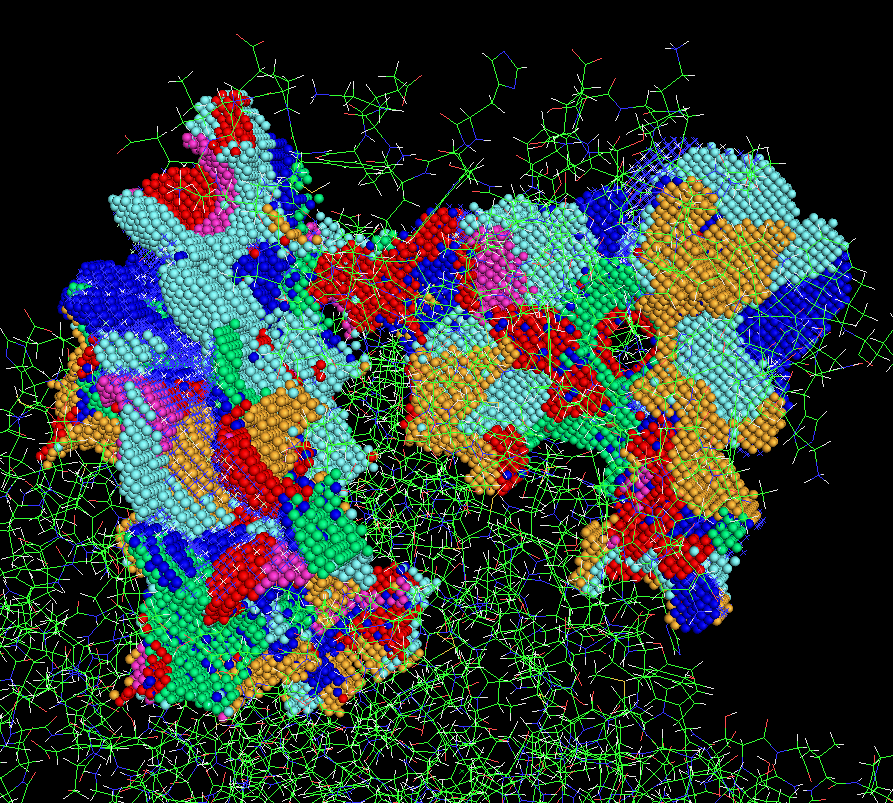
\includegraphics[width=0.6\linewidth]{pictures/mif}
		\caption{Размеченная посредством MIF наибольшая полость в структуре 1E8X из БД PDB, разные цвета обозначают тип максимального по энергии взаимодействия в этой области.}
		\label{fig:mif}
\end{figure}
\newpage
\subsection{Описание программного модуля и результаты}
Программный код на языке программирования Python 3.7 \cite{python37} и содержащий около 1800 строк \sic{обновлять} доступен в открытом репозитории по адресу \href{https://github.com/antmaxi/BSc\_thesis}{https://github.com/antmaxi/BSc\_thesis}.

Модуль состоит из четырех программ: Search.py, Drugbank.py, IsoMIF.py, Auxiliary.py, содержащих необходимые для извлечения, сравнения и поиска данных функции.
\if 0 различные функции из которых могут вызываться посредством вызова программы Search.py с соответствующими потребностям пользователя или другой программы ключами.
\fi

Состав программ:
\begin{enumerate}
	\item Search.py~--- все, кроме реализованной с помощью ПП IsoMIF, функции обработки данных для получения значений метрик схожести и скрининга по референсным данным.
	\item Drugbank.py~--- функции для извлечения, дополнения и обработки референсных данных из БД Drugbank.
	\item IsoMIF.py~--- функции для проведения поиска схожих комплексов с помощью ПП IsoMIF.
	\item Auxiliary.py~--- вспомогательные функции для работы с файловой системой, для соединения записей об одной молекуле с помощью ID различных БД (Drugbank, PubChem, Uniprot, PDB) и разных характеристик (SMILES, а/а последовательность).
\end{enumerate}

Работа модуля была протестирована на компьютере с операционной системой Ubuntu 16.04 LTS 64-bit, с процессором Intel® Core™ i9-7940X CPU @ 3.10GHz $\times$ 28 и видеокартой GeForce GTX 1080 Ti/PCIe/SSE2.
\subsubsection{Извлечение данных}
Было решено производить извлечение референсных данных из БД Drugbank, так как она является одной из наиболее полных и хорошо аннотированных БД лекарств \cite{Wishart2017} и содержит информацию не только о лигандах, но и об их мишенях вместе со ссылками на другие специфические источники информации. 

Хотя в приложении к полной БД Drugbank находятся таблицы с частью нужной для работы протокола информации (ссылки на другие БД, химические идентификаторы), было принято решение извлекать информацию напрямую из полной БД, что позволяет: 

(а) не зависеть от обновления приложений ко всей БД, которые могут запаздывать относительно общего обновления БД; 

(б) делать поиск по нужным записям/свойствам более гибким и простым для будущих модификаций и усовершенствований протокола.

При извлечении лигандов с информацией о них считалось, что лиганд подтвержден FDA, если среди указанных в БД лекарственных продуктов с его участием есть хотя бы один подтвержденный FDA. Это значит, что эта молекула в некоторых условиях безвредна для человека, так что можно включить ее в предварительный поиск лекарств. 

Поиск производился обработкой скачанной полной БД Drugbank в формате XML с помощью последовательного выбора потомков по нужным именам полей, начиная с корней всей БД. Использование сторонних модулей обработки без прямой итерации по элементам невозможно из-за большого (1,3 Гб) размера БД. Из-за этого поиск производится сравнительно дольше (3--4 минуты).

После нахождения нужной информации она сохраняется на диск компьютера, чтобы в дальнейшем можно было не просматривать всю БД при каждом запуске поиска по коэффициент подобия. Всего найдено 3220 различных лигандов, 2513 их разных мишеней и 9048 связей лиганд-мишень.


В будущем поиск такого рода можно усовершенствовать путем приоритетного рассмотрения тех пар лиганд-мишень, которые входят в подтвержденные FDA лекарства. Так же можно будет учитывать известные побочные эффекты референсных лекарств при построении прогноза перспективности входных данных для дальнейшего изучения.

\subsubsection{Сходство белков по аминокислотной последовательности}

В цикле по мишеням, извлеченным из БД Drugbank, производится сравнение АКП входного белка (можно задать по последовательности или ID Uniprot, тогда АКП запрашивается у онлайн\,--\,сервиса Uniprot) с АКП соответствующей мишени. Результатом каждого сравнения является пара чисел (подобие, идентичность), характеризующих степень похожести АКП. Затем производится сортировка полученного списка по одной из этих мер подобия, и результат выводится на экран. Причем для наиболее сходных молекул строится выравнивание для указания основных областей схожести/различия белков.

Пример использования этой функции приведен в листинге \ref{lst:fasta}
\color{black}. Была взята АКП GPCR человеческого белка родопсина, одного из важнейших белков у человека и ключевого инструмента оптогенетики. Неудивительно, что наиболее похожей мишенью из БД Drugbank оказался он же сам. Наилучшие найденные белки, как и следовало ожидать, также принадлежат семейству GPCR, но их а/к последовательности достаточно сильно отличаются от данной (падение схожести с 1843 до 318, идентичности с 348 до 156). 

\begin{lstlisting}[label={lst:fasta}, caption={Определение сходства мишеней по а/к последовательности посредством Biopython, входные данные~--- ID Uniptor человеческого родопсина из семейства GPCR.}]
In:
	get_closest_fastas_from_uniprot('P08100', path_to_data_in_fasta, k=0, align_matrix='blosum62', sim_or_ident=True)
Out:

	similarity 		identity 					name
	1392 	 	1843 	348  	lcl|BSEQ0016346|Rhodopsin
	1931 	 	318 	156 	lcl|BSEQ0010278|Cholecystokinin_receptor_type_A
	151 	 	295 	147 	lcl|BSEQ0016698|Somatostatin_receptor_type_5
	152 	 	292 	154 	lcl|BSEQ0006800|Somatostatin_receptor_type_2
	676 	 	270 	156 	lcl|BSEQ0002303|Gastrin/cholecystokinin_type_B_receptor
	1317 	 	262 	139 	lcl|BSEQ0010362|Melatonin_receptor_type_1A

	...
	
	Name = lcl|BSEQ0010278|Cholecystokinin_receptor_type_A
	Similarity=318.5, identity=156
	Matrix blosum62, number of alignments = 1
	MNGTEGPNFYVPFSNATGVVRSPFEYPQYY-LAEP-----WQFS---
	
	MLAAYMFLLIVLGFPINFLTLYVTVQHKKLRTPLNYILLNLAVADLFMVLGGFTSTLYTSLHGYFVFGPTGCNLEGFFATLGGEIAL	
	WSLVVLAIERYVVVCKPM-SNFFGENHAIMGVAFTWVMALACAAP-PLAGWSRYIP--EGLQCSCGIDYYTLKPEVNNESFVIYMFVVHFTIPMIIIFFCYGQLVFTV----------KEAAAQQQESATT------------QK---------------------------------AEKEVTRMVIIMVIAFLICWVPYASV---
	-AFYIFTHQGSNFG-PIFMTIPAFFAKSAAIYNPVIYIMMNKQFRNCMLTTICCGKNP--------LGDDEASATVSKT--------ETSQVAPA
	|....  ...|..||.|.......|..... |..|     ||..   .|....|||.|||   |.|...|....|..||..|..||.|||.||...|......|...|...|.||...|.....|...........||....|||
	...|||. |.......||....|.||........| |.  .|...|  .............|...|...|.........|.||.|.....||......          |..|.....|.|.            ||                                 |.|.|.||.|..|..|..||.|..|.    |...........| ||..........|..  ||.||..|||.||.....|..|..||        .|..|...|....        ....|.|.
	MDVVD--SLLVNGSNITPPCELGLENETLFCLDQPRPSKEWQPAVQILLYSLIFLLSVLG---NTLVITVLIRNKRMRTVTNIFLLSLAVSDLMLCLFCMPFNLIPNLLKDFIFGSAVCKTTTYFMGTSVSVSTFNLVAISLERYGAICKP
	LQSRVWQTKSHALKVIAATWCLSFTIMTPYPI--YSNLVPFTKNNNQTANMCRFLLPNDVMQQSWHTFLLLILFLIPGIVMMVAYGLISLELYQGIKFEASQKKSAKERKPSTTSSGKY
	EDSDGCYLQKTRPPRKLELRQLSTGSSSRANRIRSNSSAANLMAKKRVIRMLIVIVVLFFLCWMPIFSANAWRAYDTASAERRLSGT
	PISFILLLSYTSSCV--NPIIYCFMNKRFRLGFMATFPCCPNPGPPGARGEVGEEEEGGTTGASLSRFSYSHMSASVPPQ
	Score=318.5
	
	...
	
CPU times: user 10min 41s, sys: 1.26 s, total: 10min 42s
Wall time: 10min 43s
\end{lstlisting}

Делать прямые выводы о наличии/отсутствии общих лигандов только из выравнивания сложно, это требует отдельного поиска и анализа карманов связывания (в случае GPCR чаще всего он известен), однако наличие достаточной схожести дает основания исследовать этот вопрос для этой пары мишеней глубже. Также то, что найденные белки принадлежат тому же семейству GPCR, говорит о том, что работа функции подтверждает корректность работы функции.

Сравнение одной пары занимает от долей секунды до около 10 секунд, сравнение со всей БД порядка 10-30 минут.
\subsubsection{Сходство белков по структуре}
Список ID PDB, в которые входит белок, автоматически берется с помощью онлайн\,--\,сервиса БД Unirprot. Далее необходимо из этих структур выбрать или выделить те, в которых белок находится сам по себе, без других полипептидных цепей (так как TM-align считает схожесть для всех атомов в аминокислотах, и если белков или их частей в файле несколько, то будет обрабатывать только первую встреченную цепь; так что этот алгоритм применим только для определенного класса структур)

Для такой фильтрации списка используется ранее упоминавшееся вычисление схожести АКП с помощью ПМ Biopython. Среди встречающихся в файле цепей ищется и выделяется посредством ПМ Biopython та, которая имеет наибольшую степень 1D\,--подобия с последовательностью входного белка.

После предварительной обработки всех извлеченных из БД Drugbank белков, а также протеомов человека, крысы и мыши, искомый белок с помощью TM-align сравнивается с выделенными структурами для одного из упомянутых наборов белков. Они сортируются по вычисленным TM-score и выводятся на экран.
\subsubsection{Сходство лигандов по структуре}
Поиск по ID SMILES:

Из БД Drugbank извлекаются соответствующие ID SMILES подтвержденных FDA лигандов. Информация дополняется извлеченными из БД PubChem (\href{https://pubchem.ncbi.nlm.nih.gov}{https://pubchem.ncbi.nlm.nih.gov}) идентификаторами тех лигандов, у которых нет ID SMILES в БД Drugbank, но имеющих запись в БД PubChem.

Далее, с помощью ПМ RDkit строятся и сравниваются молекулярные отпечатки, вычисляется коэффициент Танимото между ними, приводя к отсортированному по степени подобия списку подтвержденных FDA лигандов. Пример приведен в листинге \ref{lst:smiles-fing}.

\begin{lstlisting}[language=Python, label={lst:smiles-fing}, caption={Сходство лигандов по текстовым молекулярным отпечаткам с помощью ПМ RDkit для входных данных~--- SMILES структуры молекулы.}]
In:
	smiles = get_smiles_from_name_from_pubchem(name_lig, root)
	df = get_closest_smiles_names(smiles, root, 5)
Out:
	Name  					Tanimoto coeff			 Drugbank ID 		Fingerprint type
	0    Losartan        1.000000     DB00678            maccs
	1  Olmesartan        0.735294     DB00275            maccs
	2   Valsartan        0.690141     DB00177            maccs
	3  Irbesartan        0.681159     DB01029            maccs
	4  Crizotinib        0.657143     DB08865            maccs
CPU times: user 2.66 s, sys: 7.99 ms, total: 2.67 s
Wall time: 2.66 s
\end{lstlisting}

Действительно, вводом был ID Uniprot Лосартана, а Олмесартан является его обратным агонистом, то есть связывается с той же мишенью (AGTR1), так что такой поиск мог бы это выявить, не будь это известно заранее. Названия остальных лигандов из списка также указывают на их схожесть в реальности.

Поиск по структуре в формате SDF:

С сайта БД Drugbank скачивается файл со структурами всех лигандов в формате SDF, из него по ID в БД Drugbank извлекаются структуры подтвержденных FDA лигандов. Затем по этим структурам получаются молекулярные отпечатки, вычисляется коэффициент Танимото между ними, результируя в искомом списке. Пример приведен в листинге \ref{lst:sdf-fing}.

\begin{lstlisting}[language=Python, label={lst:sdf-fing}, caption={Сходство лигандов по топологическим молекулярным отпечаткам с помощью ПМ Open Babel для входных данных~--- SDF структуры молекулы.}]
In: 
	get_closest_ligands_from_3d_structure(path_to_structure, path_to_sdf_approved, root,
fptype='maccs', number_to_print=5)
Out:
	                                 name  
	481                          Losartan  
	132                        Olmesartan  
	923                        Fomepizole  
	1110                     Tromethamine  
	947                       Gemfibrozil  
	
																smiles  													similarity  \
	481   CCCCC1=NC(Cl)=C(CO)N1CC1=CC=C(C=C1)C1=CC=CC=C1...    1.000000   
	132   CCCC1=NC(=C(N1CC1=CC=C(C=C1)C1=C(C=CC=C1)C1=NN...    0.677469   
	923                                          CC1=CNN=C1    0.531250   
	1110                                       NC(CO)(CO)CO    0.531250   
	947                  CC1=CC(OCCCC(C)(C)C(O)=O)=C(C)C=C1    0.522267 
 

CPU times: user 1.87 s, sys: 7.68 ms, total: 1.88 s
Wall time: 1.88 s
\end{lstlisting}

Здесь также Олмесартан занял второе место, что подтверждает работу функции.

Время поиска по молекулярным отпечатком для всей БД около 1-3 сек.
\subsubsection{Сходство сайтов связывания}
Для сравнения комплекса из входных данных с референсными комплексами необходимо каким-то образом получить их структуры. С этой целью для лиганда и мишени строятся два списка ID PDB, включающих в себя их. 

Для мишени список составляется просто по ID Uniprot c помощью запросов к онлайн\,--\,сервису БД Uniprot, позволяющего находить соответствующие данному белку ID PDB (при этом может случиться, что в этих структурах находится белок как сам по себе, так и в комплексе с некоторым лигандом). 

Для лиганда по его SMILES (у 1939 из 3220 извлеченных лигандов SMILES имеется) ищутся и сохраняются для будущих запусков его ID PDB, в которых есть похожая на него структура. Для этого нужно ввести достаточный уровень коэффициент Танимото или же указать шаг, с которым этот коэффициент будет уменьшаться начиная с 1 до тех пор, пока не будет найдена хотя бы одна структура в БД PDB или не будет достигнуть задаваемый максимальный уровень похожести. При фиксированном шаге в 0,05 время поиска всех PDB (определяется главным образом временем получения ответа с сайта БД Uniprot) занимает для различных максимальных уровней: 1.0 (то есть поиск точных совпадений)~-- около 30 минут, 0.9~-- около 40 минут. С фиксированным уровнем подобия результаты: 0.9~-- около 35 минут, 0.8~-- около 45 минут. Стоит заметить, что также существуют таблицы, в которых эти списки уже составлены, но для некоторых заданных уровней подобия. Нас же подход позволяет гибко настраивать параметры поиска в зависимости от требуемой точности и располагаемых ресурсов.

Затем находятся и также общие элементы списков ID PDB для мишени и лиганда.

Корректность работы этой части была проверена взятием случайного лиганда (ацетазоламида) и одной и его мишеней (карбоангидразы 4). Три наиболее близкие лиганду общие структуры в PDB и их уровни подобия лигандов совпадают с данными в приложенной к БД Drugbank таблице. Однако, в этой таблице указаны только 3 лучшие структуры по сходству к лиганду, а наш метод позволяет найти нужное нам количество с необходимой точностью, так что здесь, как и с первичным поиском подтвержденных лигандов, стратегия самостоятельного поиска вместо простой обработки приложений к БД дает свои плоды.

Далее, простым циклом по референсным парам лиганд-мишень можно получить для каждого комплекса коэффициент его сходства с исходным комплексом и затем отсортировать результат по убыванию подобия.

В качестве сторонних программ, вычисляющих коэффициенты схожести, используются ПП IsoMIF и TM-align. Находятся коэффициенты подобия карманов связывания для всех найденных референсных структур комплексов и входного комплекса, и выводятся наиболее похожие.

Для одной пары полостей время построения MIF обычно около \linebreak 1--3 мин, время вычисления IsoMIF около 3--5 мин, остальные части этого поиска длятся пренебрежимо мало. По всей БД поиск произведен не был из-за слишком большого времени работы. Предлагается в дальнейшем усовершенствовать протокол добавлением параллельных версий наиболее ресурсоемких и времязатратных частей.

Для одной пары полостей время работы TM-align составляет несколько секунд, для всей БД около 20 минут.

\newpage
\section{Заключение}
Построен протокол поиска подобных и соответствующих подтвержденным FDA лигандов/мишеней/комплексов по нескольким типам входных данных с использованием различных способов вычисления коэффициентов подобия: по 1D\,--, 2D\,--, 3D\,--\,структурам. Работа протокола проверена и задокументирована, программный код и примеры использования опубликованы в открытом доступе.

Из-за своей модульной структуры в будущем протокол может дополняться новыми вариантами нахождения меры схожести. Также на его основе с применением машинного обучения могут быть построены более сложные методы поиска, учитывающие несколько различных метрик подобия. Усовершенствование протокола может быть дополнительно осуществлено учетом данных о побочных эффектах известных лекарств, которые могут влиять на предсказания эффектов найденных кандидатов. Также может быть реализован удобный пользовательский интерфейс работы в командной строке или графическом режиме.


\newpage
\printbibliography[heading=bibintoc, title=Список использованных источников]

\end{document}